% About 2.5 pages
% Up to 2 references

The core methodology this paper will implement is a purely quantitative mix between comparative and evaluative research, with the generation of data being slightly exploratory.

\subsection{Testing and Evaluation Framework}\label{sec:testing-framework}

This section will present the proposed Monte Carlo-based data generation, describe the implementation of the testing and evaluation framework and discuss the measures of effectiveness used for comparison.

\subsubsection{Data Generation with Monte Carlo Simulation and Randomised Algoritms}

Due to the previously discussed ethical and privacy issues with real-world data collection and impracticality of setting up a real-world 802.11 study, a seemingly simple solution is to instead generate the data through Monte Carlo simulation.
Additionally, while there are plenty of existing datasets, they do not contain all the fields required for the application of each of the independent methods.
Because of this, the implementation of a Monte Carlo simulation to generate location data representative of devices with, and without, MAC randomisation would not only be useful for this study, but also future research (potentially in related fields).
This is combined into a testing and evaluation framework that enables the modular insertion or removal of the methods shown in Figure 3 (plus the hybrid model with all of them combined).

Pinpointing location with 802.11 is a more complex technical issue than the implementation of triangulation alone.
Much like with GPS, the indoor environment presents localisation difficulty due to walls and other obstructions.
A typical existing wireless infrastructure may consist of one access point per floor, or, at best, one per room.
If such a system was transformed to include an IPS without additional hardware modification, it would result in high inaccuracy when estimating the location of a device.
Because of this, the Monte Carlo simulation will emulate an ideal testing environment, where there are multiple access points in a single room.

The Monte Carlo method is a class of algorithms which leverage random sampling to obtain numerical results~\cite{raychaudhuri2008}.
They are well-suited to simulating physical models due to their near-nondeterministic nature.
This makes them ideal for simulating physical-layer characteristics such as those used by implicit identifier fingerprinting.
Additionally, they can be used to simulate the frame emission times required by the timing attack.

 simulations is the employment of random-based algorithms to generate both true and randomised MAC addresses.
These can then be used by the timing attack as part of its fingerprinting and be sent for MAC vendor analysis.

Finally, each simulation (whether considering one or more devices) is run a fixed number of times.
The exact number of times they are run is determined experimentally trough trial and error until the results converge to within a pre-determined error margin.

\subsubsection{Software Framework}

Each de-randomisation technique is independently implemented as a module extending a \texttt{DerandomisationTechnique} abstract base class, specifying the location data fields they require as input from the framework.
At runtime, through dependency injection, the framework provides the requested data (and continues to update it as the simulation runs).
It then calls to an interface method implemented by the technique to return the MAC addresses.

To guarantee more valid, truthful location-data output from the Monte Carlo simulation, its hyperparameters and probability distributions are fine-tuned by running the independent techniques and tweaking them to closely match the results obtained in their respective papers.

The implementation provided by the framework of the 802.11 protocol is designed to enable modularity.
For the reasons mentioned earlier, this enables testing of how well the various techniques work on different versions of the 802.11 protocol.
An object-oriented approach is proposed whereby an abstract base class, \texttt{Simulated80211}, is inherited by concrete classes which implement the respective version of 802.11 (for example, \texttt{Simulated80211b} for the 1999 version, or \texttt{Simulated80211ax} for the 2021 version).
It is within these concrete classes that the Monte Carlo simulation and randomised algorithms are implemented.
This is then further abstracted to have \texttt{Simulated80211} extend the abstract base class \texttt{WirelessProtocol}, allowing any protocol to be used.
Because of this, the concrete implementation of the protocol corresponding to the one being tested (or used for evaluation) is instantiated at runtime, and can be freely swapped out as required (even for a real-world source).

With this in mind (and using the separation of concerns principle), the concepts of premises (\texttt{Premises}), devices (\texttt{Device}), APs (\texttt{AccessPoint}) and IPS software (\texttt{IpsSoftware}) are defined as different entities.
In the 3D model, for simplicity, premises are represented by a rectangular cuboid of arbitrary size, and both APs and devices are represented by a single point within the bounds of the premises.
Implementation-wise, a \texttt{Premises} only stores its bounding-box, a \texttt{Device} and \texttt{AccessPoint} both store a three-dimensional position vector and a \texttt{WirelessProtocol} and \texttt{IpsSoftware} stores a \texttt{DerandomisationTechnique} instance.
All of these are externally managed by a \texttt{SimulationManager}.
The manager maintains a list of \texttt{EvaluationMetric} instances which use the results to calculate the metrics listed below.
Because the manager has access to both the simulated results and true location assignments, it sends them into each \texttt{EvaluationMetric} and outputs the results.

\subsubsection{Measure of Effectiveness}

The primary measure of how effective each method is will be based upon the percentage of devices successfully tracked over discrete time frames.
The reason for using this is because it closely matches the real-world application of tracking users’ locations across space and time.
In addition to their use in simulation calibration, the other metrics from the original papers can be used for the hybrid system and compared as a supplement to the primary spatio-temporal measure of success.
Finally, as the framework is a controlled environment, the simulation manager is able to undertake performance profiling for speed and memory usage on the simulated techniques.
This performance information is also useful knowledge for real-world application because it can be used to determine required hardware specifications.

\subsection{Hybrid System}\label{sec:hybrid-system}

This section will go into more detail on how the three MAC de-randomisation techniques fit together to form the hybrid system and how it fits with the software framework.

\subsubsection{Overview}

Figure~\ref{fig:solutionstack} shows a high-level diagram-description demonstrating the modularity and the layers at which each technique resides in the OSI model.
Each layer is directly related to the data it requires: implicit identifier fingerprinting requires low-level parameters such as packet size, (encrypted) packet data and 802.11 options, timing attacks require low-level parameters such as probe request data and IAT, and higher-level parameters like MAC address, and this implementation of MAC vendor analysis requires only the broadcast MAC address.

\begin{figure}[!ht]
    \centering
    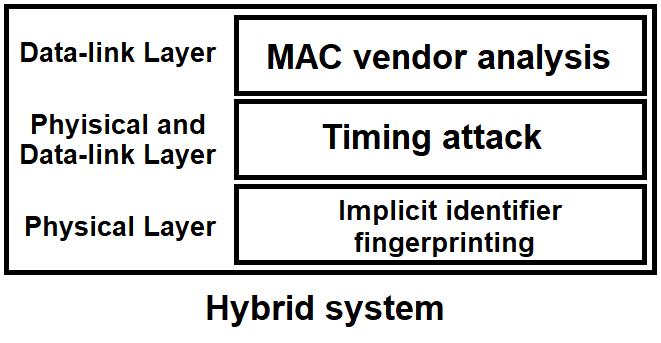
\includegraphics[scale=0.25]{figures/solutionstack.png}
    \caption{Illustration of the proposed hybrid system, and the OSI layers it encompasses.}
    \label{fig:solutionstack}
\end{figure}

\subsubsection{Software Implementation}

The modular approach described in~\nameref{sec:testing-framework} continues to apply to the hybrid system.
The concrete class \texttt{HybridTechnique} extends \texttt{DerandomisationTechnique} and contains one field for each independent technique.
As it extends the \texttt{DerandomisationTechnique} base class, it can be substituted in at runtime as if it were its own technique.
All it has to do is implement a way to pass required arguments and the simulated location-data down to the respective techniques.
